\section{Shuffle Optimization}
In this section, we present the detailed methodologies to achieve three design goals. The memory copy is used to decouple shuffle from execution. Shuffle data is pre-fetched without tasks launching with the pre-scheduling result by heuristic MinHeap. And all shuffle data is managed outside DAG framework by SCache, which provides a universal cross-framework optimization.
We choose Spark as the representative of DAG computing framework to implement our optimization.

\begin{figure}
	\centering
	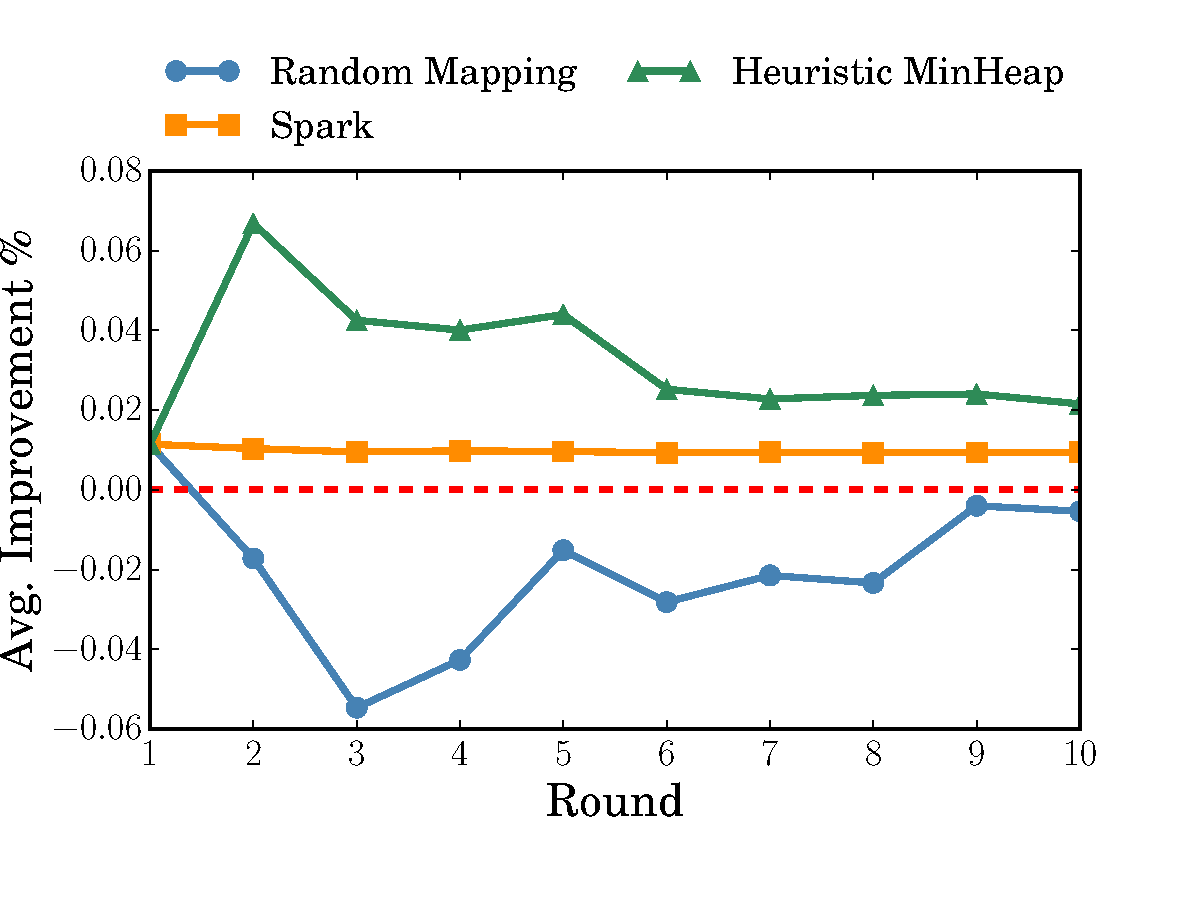
\includegraphics[width=0.9\linewidth]{fig/sim}
	\caption{Stage Completion Time Improvement of OpenCloud Trace}
	\label{fig:sim}
\end{figure}

\subsection{Decouple Shuffle from Execution}
On the map side, map tasks partition the output data according to the pre-defined partitioner. More specifically, partitioner takes a set of key-value pairs as input. And then it calculates the partition number of a key-value pair by applying pre-defined the partition function to the key. After that it puts the key-value pair into the corresponding data blocks. Each of them contains the key-value pairs for one partition. At last, they will be flushed to disk. The decoupling starts right here. To prevent from the synchronized disk write holding the slot, we use memory copy to hijack shuffle data from Spark executor's JVM space. By doing this, a slot can be released as soon as it finishes CPU intensive computing. After that, shuffle data is managed outside the DAG framework. The pre-scheduling can be performed to start pre-fetch after enough shuffle data is collected.

On the reduce side, shuffle read is decoupled by pre-fetching shuffle data to local memory after pre-scheduling before reduce tasks start.

To this end, all I/O operations are managed outside of the DAG framework, and the slot is occupied only by the CPU intensive phase of task.
\begin{figure}
	\centering
	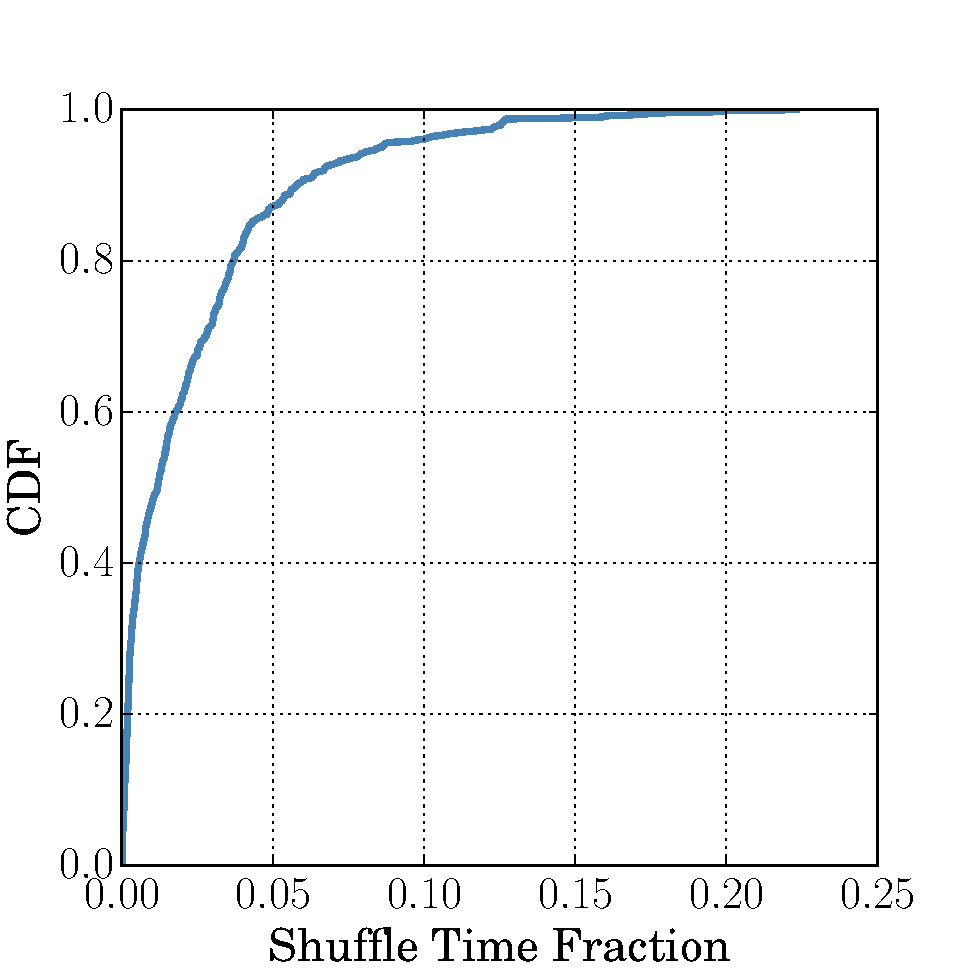
\includegraphics[width=0.75\linewidth]{fig/reduce_cdf}
	\caption{Shuffle Time Fraction CDF of OpenCloud Trace}
	\label{fig:cdf}
\end{figure}
\subsection{Pre-schedule with Application Context}
The main challenge toward the optimization is how to pre-schedule the reduce tasks without launching. The task --- node mapping is decided until tasks are scheduled by scheduler of DAG framework. But as soon as they are scheduled, slots will be occupied to launch them. On the other hand, shuffle data cannot be pre-fetched without knowing the node and tasks mapping.
To get rid of this dilemma, we propose a co-scheduling scheme. That is, the task --- node mapping is established ahead of DAG framework scheduler, and then enforce the mapping result to DAG scheduler while doing the real scheduling.

To evaluate the impact of different pre-scheduling schemes, we use trace from OpenCloud \cite{opencloudtrace} for the simulation. The baseline (red dot line in Figure \ref{fig:sim}) is the stage completion time under Spark default scheduling algorithm. And then we remove the shuffle read time of each task, and do the simulation under three different schemes: random mapping, Spark FIFO, and our heuristic MinHeap.

% We explore several pre-scheduling schemes in different scenarios, and evaluate the performance calculating the improvement of reduce tasks completion time with trace of OpenCloud \cite{opencloudtrace}. We first emulate the scheduling algorithm of Spark to schedule the reduce tasks of one job, and take the bottleneck of the task set as the completion time. Then we remove the shuffle read time as the assumption of shuffle data pre-fetch and emulate under different schemes. The result is shown in \ref{fig:sim}.
% \begin{figure*}
% 	\centering
% 	\begin{minipage}{0.34\linewidth}
% 		\begin{figure}[H]
% 			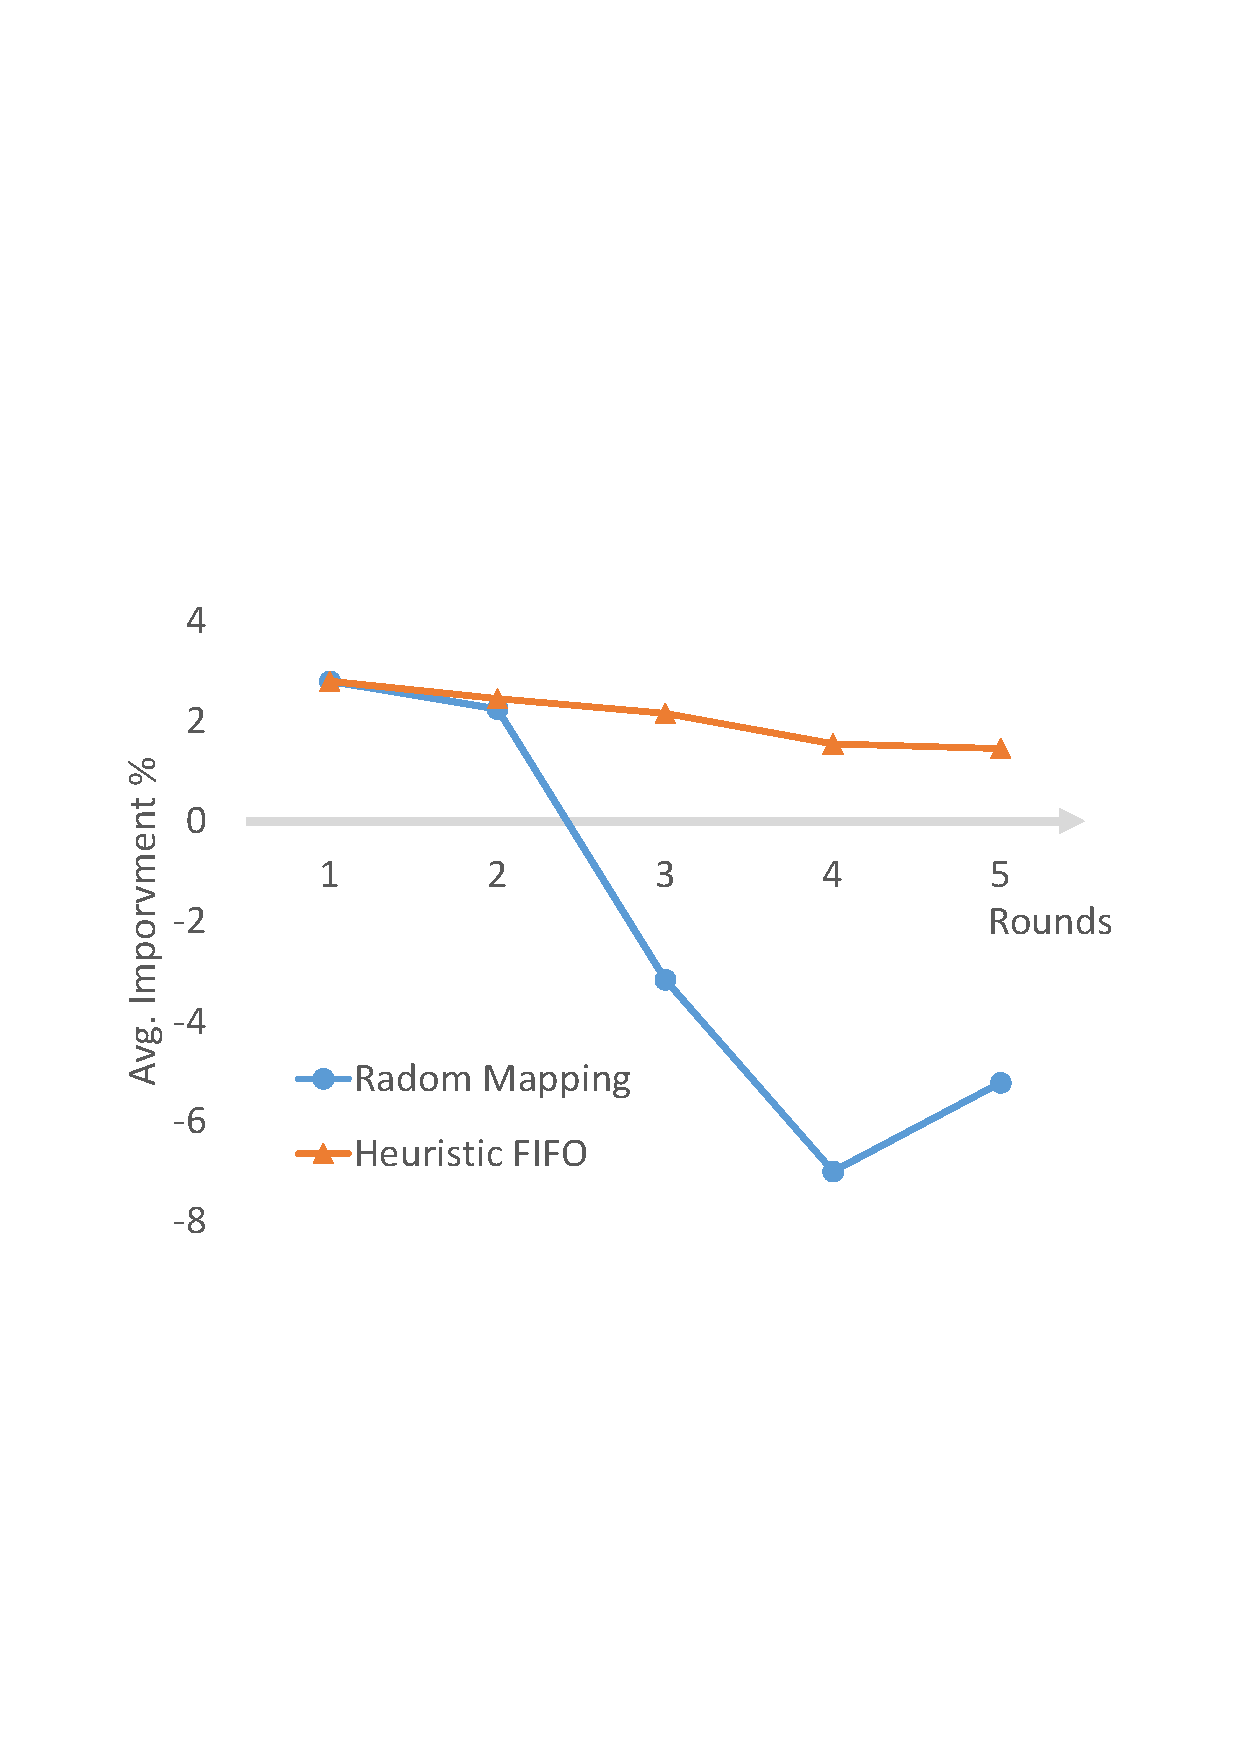
\includegraphics[width=\textwidth]{fig/shuffle_size}
% 			\caption{Shuffle Size Comparing with Input Size}
% 			\label{fig:shuffle_size}
% 		\end{figure}
% 	\end{minipage}
% 	\begin{minipage}{0.65\linewidth}
% 		\begin{figure}[H]
% 			\begin{subfigure}{0.5\textwidth}
% 				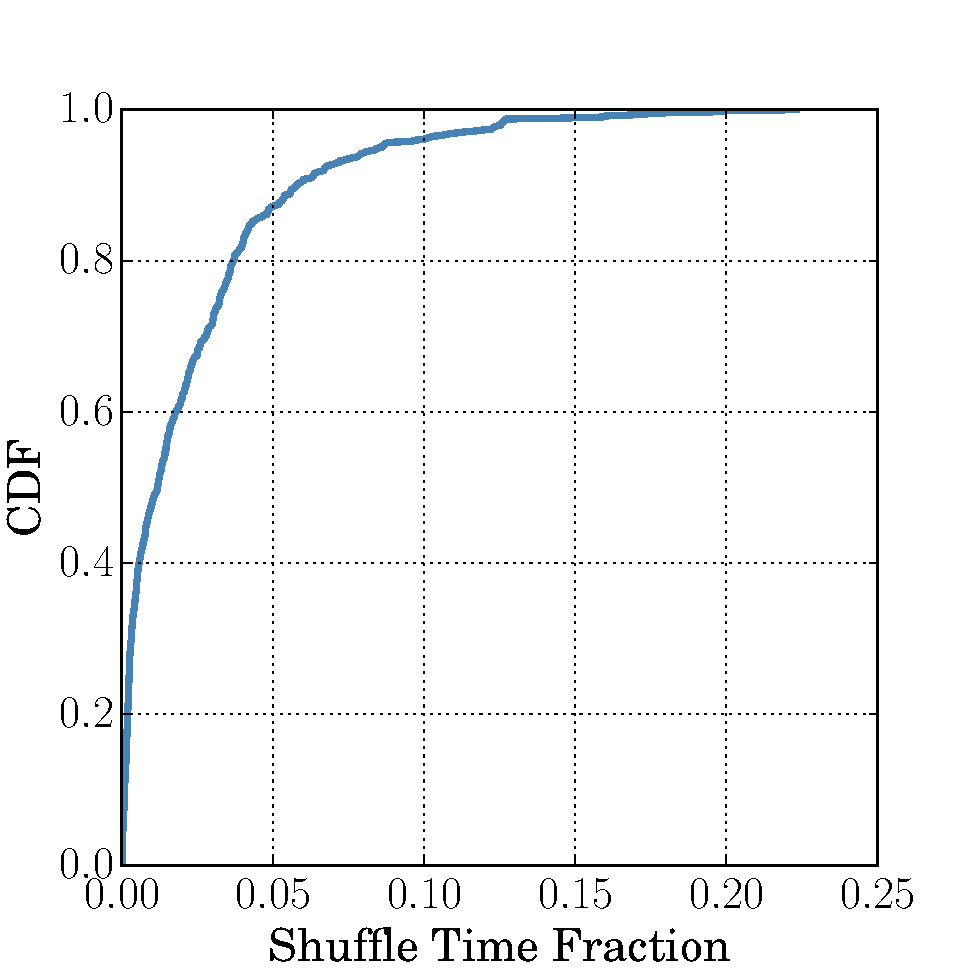
\includegraphics[width=\linewidth]{fig/reduce_cdf}
% 				\caption{Shuffle Time Fraction CDF}
% 				\label{fig:cdf}
% 			\end{subfigure}	
% 			\begin{subfigure}{0.5\textwidth}
% 				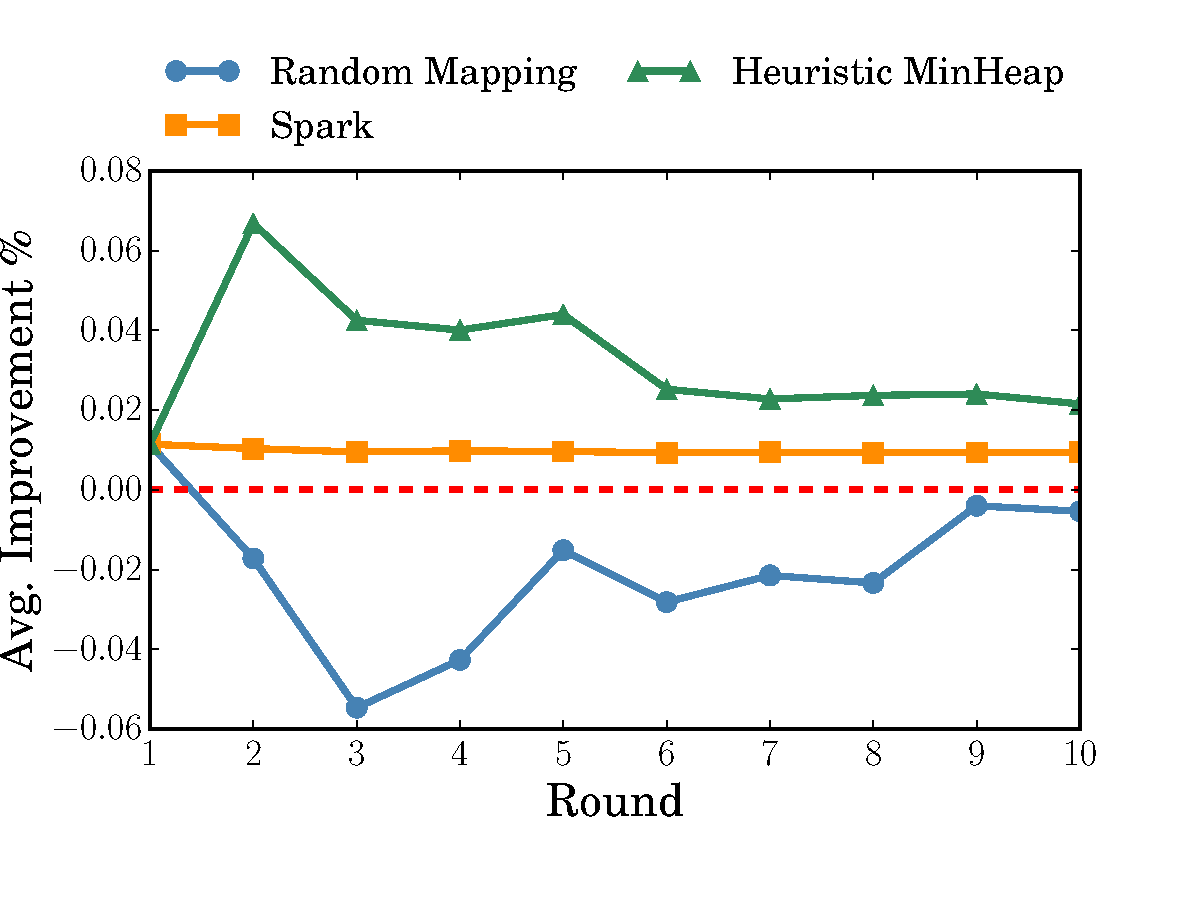
\includegraphics[width=\linewidth]{fig/sim}
% 				\caption{Stage Completion Time Improvement}
% 				\label{fig:sim}
% 			\end{subfigure}	
% 			\caption{Emulate Result of OpenCloud Trace}
% 		\end{figure}
% 	\end{minipage}
% \end{figure*}
% \begin{figure}



Note that most of the traces from OpenCloud is shuffle-light workload as shown in Figure \ref{fig:cdf}. The average shuffle read time is 2.3\% of total reduce completion time.

\subsubsection{Failure of Random Mapping}\label{randomassign}
The simplest way of pre-scheduling is mapping tasks to different nodes evenly.  As shown in Figure \ref{fig:sim}, Random mapping works well when there is only one round of tasks. But the performance collapses as the round number grows. It is because that data skew commonly exists in data-parallel computing \cite{skewtune, reining, gufler2012load}. Several heavy tasks might be assigned on the same node. This collision then slows down the whole stage, which makes the performance even worse than the baseline. In addition, randomly assigned tasks also ignore the data locality between shuffle map output and shuffle reduce input, which might introduce extra network traffic in cluster.


\subsubsection{Shuffle Output Prediction}\label{shuffleprediction}
The failure of random mapping was obviously caused by application context (e.g. shuffle data size) unawareness. To avoid the `bad' scheduling results, we have to leverage the application context as assistance. The optimal schedule decision can be made under the awareness of shuffle dependencies number, partition number and shuffle size for each partition. The first two of them can be easily extracted from DAG information. To achieve a better scheduling result, the shuffle size for each partition should be predicted during the initial phase of map tasks.

According to the DAG computing process, the shuffle size of each reduce task is decided by input data, map task computation, and hash partitioner. For each map task, it produces a data block for each reduce task. The size of each reduce partition can be calculated $reduceSize_i = \sum_{j=0}^{m} {BlockSize_{ji}}$. $m$ is the number of map tasks. $BlockSize_{ji}$ represents the size of block which is produced by \textit{map task j} for \textit{reduce task i}(e.g., block `1-1' in Figure \ref{fig:shuffle}). For Hadoop MapReduce, the $BlockSize_{ji}$ can be predicted with decent accuracy by liner regression model based on observation that the ratio of map output size (e.g. map output in Figure \ref{fig:shuffle}) and input size is invariant given the same job configuration \cite{ishuffle, predict}.

But the sophisticated DAG computing framework like Spark introduces more uncertainties. For instance, the reduce stage in Spark has more number of tasks than Hadoop MapReduce. More importantly, the customized partitioner might bring huge inconsistency between observed map output blocks distribution and the final reduce input distribution as presented in Figure \ref{fig:dis}. We use different datasets with different partitioners and normalize three sets of data to $0-1$ to fit in one figure. In Figure \ref{fig:hash_pre}, we use a random input dataset with the hash partitioner. In Figure \ref{fig:range_pre_sample}, we use a skew dataset with the range partitioner of Spark \cite{sparksource}.
The observed map outputs are randomly picked. As we can see, in hash partitioner, the distribution of observed map output is close to the final reduce input distribution. The prediction results also turn out to be good. However, the huge inconsistency between final reduce distribution and observed distribution results in a deviation in linear regression model.
% Several map outputs (marked as Map Output in Figure \ref{fig:shuffle}) are picked as observation objects to train the model and than predict the final reduce distribution.

\begin{equation}
\label{equationsample}
\begin{aligned}
	reduceSize_i = {\displaystyle\sum_{j=0}^{m} {partitionSize_j \times \frac{sample_i}{s \times p}}} \\
	{\left( m = \text{partition number of input data} \right)}
\end{aligned}
\end{equation}

To handle this inconsistency, we introduce another methodology named weighted reservoir sampling. The classic reservoir sampling is designed for randomly choosing \textit{k} samples from \textit{n} items, where \textit{n} is either a very large or an unknown number \cite{reservoir}. For each partition of map task, we use reservoir sampling to randomly pick $s \times p$ of samples, where $p$ is the number of reduce tasks and $s$ is a tunable number. The number of input data partition and reduce tasks can be easily obtained from the DAG information. In Figure \ref{fig:range_pre_sample}, we set $s$ equals $3$. After that, the map function is called locally to process the sampled data (\textit{sampling} in Figure \ref{fig:shuffle}). The final sampling outputs are collected with the size of each map partition which is used as weight for each set of sample. For each reduce, the predicted size $reduceSize_i$

As we can see in Figure \ref{fig:range_pre_sample}, the result of sampling prediction is much better even in a very skew scenario. The variance of the normalized between sampling prediction and reduce distribution is because the standard deviation of the prediction result is relatively small compared to the average prediction size, which is $0.0015$ in this example. Figure \ref{fig:prediction_relative_error} further proves that the sampling prediction can provide precise result even in the dimension of absolute shuffle partition size. On the opposite, the result of linear regression comes out with huge relative error.

During the phase of shuffle output prediction, the composition of each reduce partition is calculated as well for a better locality scheduling. We define $prob_i$ as

\begin{equation}
\label{equationsample}
\begin{aligned}
	prob_i = \max_{0 \leq j \leq n} \left( BlockSize_{ji} / size_i \right)\\
    {\left( n = \text{partition number of input data} \right)}
\end{aligned}
\end{equation}

\begin{minipage}{\columnwidth}
\begin{algorithm}[H]
\caption{Heuristic MinHeap Scheduling for Single Shuffle}
\label{hminheap}
	\begin{algorithmic}[1]
	\small
	\Procedure{schedule}{$m, h, p\_reduces$}
		\State $R\gets$ sort $p\_reduces$ by size
		\State $M\gets$ mapping of host id in $h$ to reduce id and size
		\State $rid\gets$ len$\left(R\right)$
		\Comment{Current scheduled reduce id}
		\While{$rid \geq 0$}
		\Comment{Schedule reduces by MinHeap}
		\State Update $M\left[0\right].size$
		\State Assign $R\left(rid\right)$ to $M\left[0\right]$
		\State sift\_down$\left(M\left[0\right]\right)$
		\State
		\Comment{Use min-heap according to size in $M$}
		\State $rid\gets rid-1$
		\EndWhile
		\State $max\gets$ maximum size in $M$
		\State $rid\gets$ len$\left(R\right)$
		\While{$rid \geq 0$}
		\Comment{Heuristic swap by locality}
		\State $prob\gets$ max composition portion of $rid$
		\State $norm\gets \left(prob-1/m\right)/\left(1-1/m\right)/10$
		\State
		\Comment{Use $norm$ to limit the performance degradation in tasks swap}
		\State $t\_h\gets$ host that produces $prob$ data of $rid$
		\State $c\_h\gets$ current assigned host by MinHeap
		\If{$t\_h == c\_h$}
			\State Seal the assignment of $rid$ in $M$
		\Else
			\State swap\_tasks$\left(rid, c\_h, t\_h, max, norm\right)$
		\EndIf
		\State $rid\gets rid-1$
		\EndWhile
		% \Comment{$m$ is the number of input data}
		% \Comment{$r$ is partition number of reduces}
		% \Comment{$hosts$ is array of (hostid, partitionids[], size)}
		% \Comment{$c$ is $r*m$ array of composition data}
		% \Comment{$pSize$ is $r$ size array of predicted size of reduces}
		\Return $M$
	\EndProcedure
	\Procedure{swap\_tasks}{$rid, c\_h, t\_h, max, norm$}
	\State $num\gets$ number of reduces
	\State selected from $t\_h$ that $total\_size$ won't
	\State make both $c\_h$ and $t\_h$ exceed $\left(1+norm\right)*max$
	\State after swapping
	\If{$num == 0$}
		\State return
	\Else
		\State \# Swap $nums$ reduces with $rid$ between $c\_h$ and $t\_h$
		\State \# Update size of $t\_h$ and $c\_h$
	\EndIf
	\EndProcedure
	\end{algorithmic}
\end{algorithm}
\end{minipage}

However, sampling prediction trade accuracy with extra overhead in DAG computing process. we will evaluate the overhead in the Section \ref{evaluation}. Though in most cases, the overhead is acceptable, the sampling prediction will be triggered only when the range partitioner or customized non-hash partitioner occurs.

\subsubsection{Heuristic MinHeap Scheduling}\label{h-minheap}
In order to achieve the uniform load on each node while reducing the network traffic, we present a heuristic MinHeap (\ref{hminheap}) as the scheduling algorithm for single shuffle. It takes predicted shuffle distribution, locality information and DAG information as input. Unlike the na\"{i}ve Spark scheduling algorithm, these information helps the scheduler make a more balanced task --- node mapping, which accelerates the reduce stage. This is the by-product optimization harvested from shuffle size prediction.

As for the input of $schedule$ function in Algorithm \ref{hminheap}, $m$ is the partition number of input data; $h$ is the array of nodes ID in cluster; $p\_reduces$ is the predicted reduce matrix. Each row in $p\_reduces$ contains $r\_id$ as reduce partition ID; $size$ as predicted size of this partition; $prob$ as the maximum composition portion of reduce data; $host$ as the node ID that produce the maximum portion of reduce data. As for $M$, it is a matrix consists $hostid$, $size$ (total size of reduce data on this node) and an array of $r\_id$.

This algorithm can be divided into two rounds. In the first round (i.e., the first $while$ in Algorithm \ref{hminheap}), the reduce tasks are first sorted by size in a descending order. For hosts, we use a min-heap to maintain the priority by size of assigned tasks. So that the heavy tasks can be distributed evenly in the cluster.
% After the scheduling, the completion time of reduce stage is close to the optimal. \textcolor{red}{may need to add math prove between this and optimal}.
In the second round, the task --- node mapping will be adjusted according to the locality. The closer $prob$ is to $1/m$, the more evenly this reduce partition is produced in cluster. For a task which contains at most $prob$ data from $host$, the normalized probability $norm$ is calculated as a bound of performance degradation. This normalization can ensure that more performance can be traded when the locality level increases. But the degradation of performance will not exceed 10\% (in extreme skew scenarios). If the assigned host($c\_h$ in Algorithm \ref{hminheap}) is not equal to the $host$ ($t\_h$ in algorithm \ref{hminheap}), than $swap\_tasks$ will be triggered.
%it has the $nor$ probability to trigger a tasks swap between two hosts.
Inside of the $swap\_tasks$, tasks will be selected and swapped without exceeding the performance tradeoff threshold ($\left(1+norm\right)*max$). We use the OpenCloud \cite{opencloudtrace} trace to evaluate Heuristic MinHeap. Without swapping, the Heuristic MinHeap can achieve a better performance improvement (average 5.7\%) than the default Spark FIFO scheduling algorithm (average 2.7\%). The test bed evaluations are presented in Section \ref{evaluation}.
% In the case of extreme skew scenario, such as Figure \ref{fig:range_pre_sample}, Heuristic MinHeap trades about 0.05\% percent of stage completion time for 99\% reduction of shuffle data transmission through network by heuristicly swapping tasks.

\begin{figure}
	\centering
	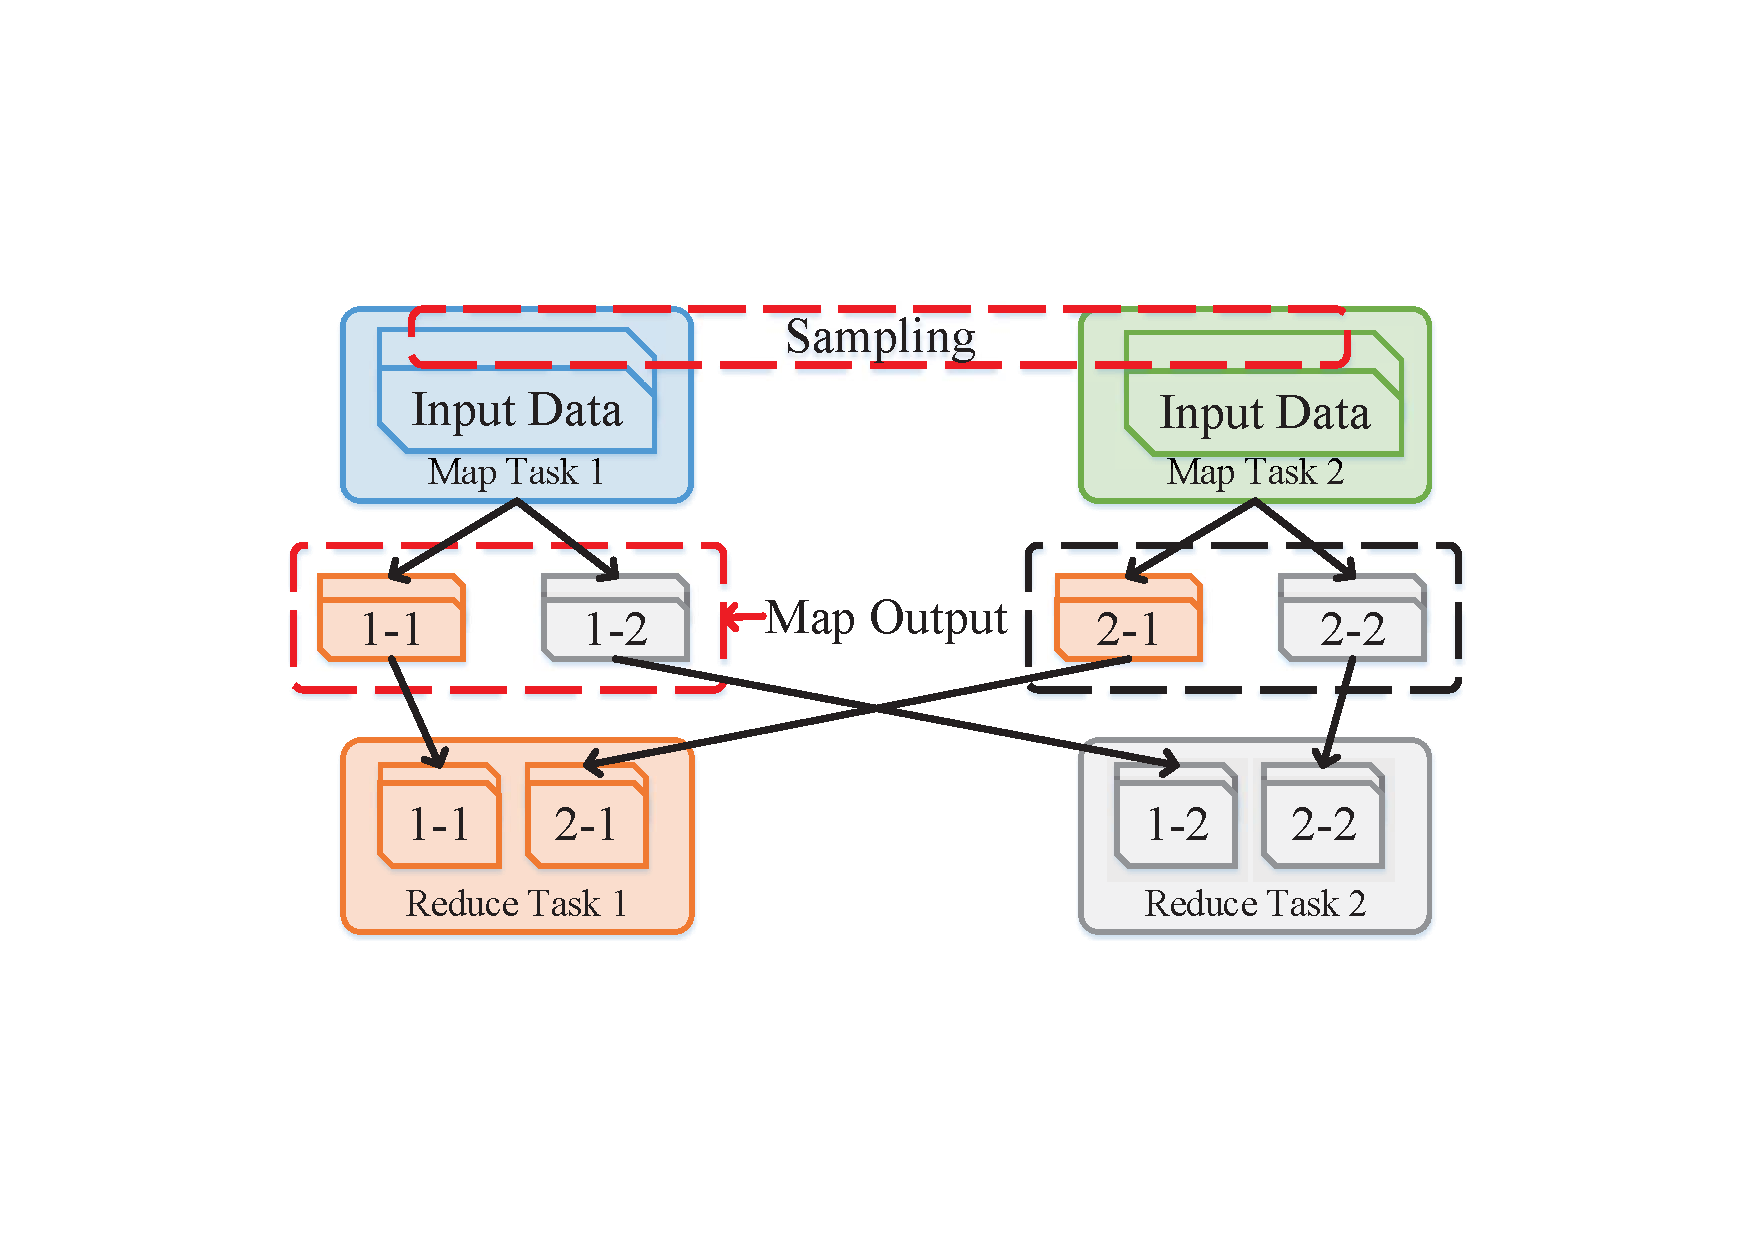
\includegraphics[width=0.9\linewidth]{fig/shuffle}
	\caption{Shuffle Data Prediction}
	\label{fig:shuffle}
\end{figure}

\begin{figure*}
	\centering
	\begin{subfigure}[b]{0.32\linewidth}
		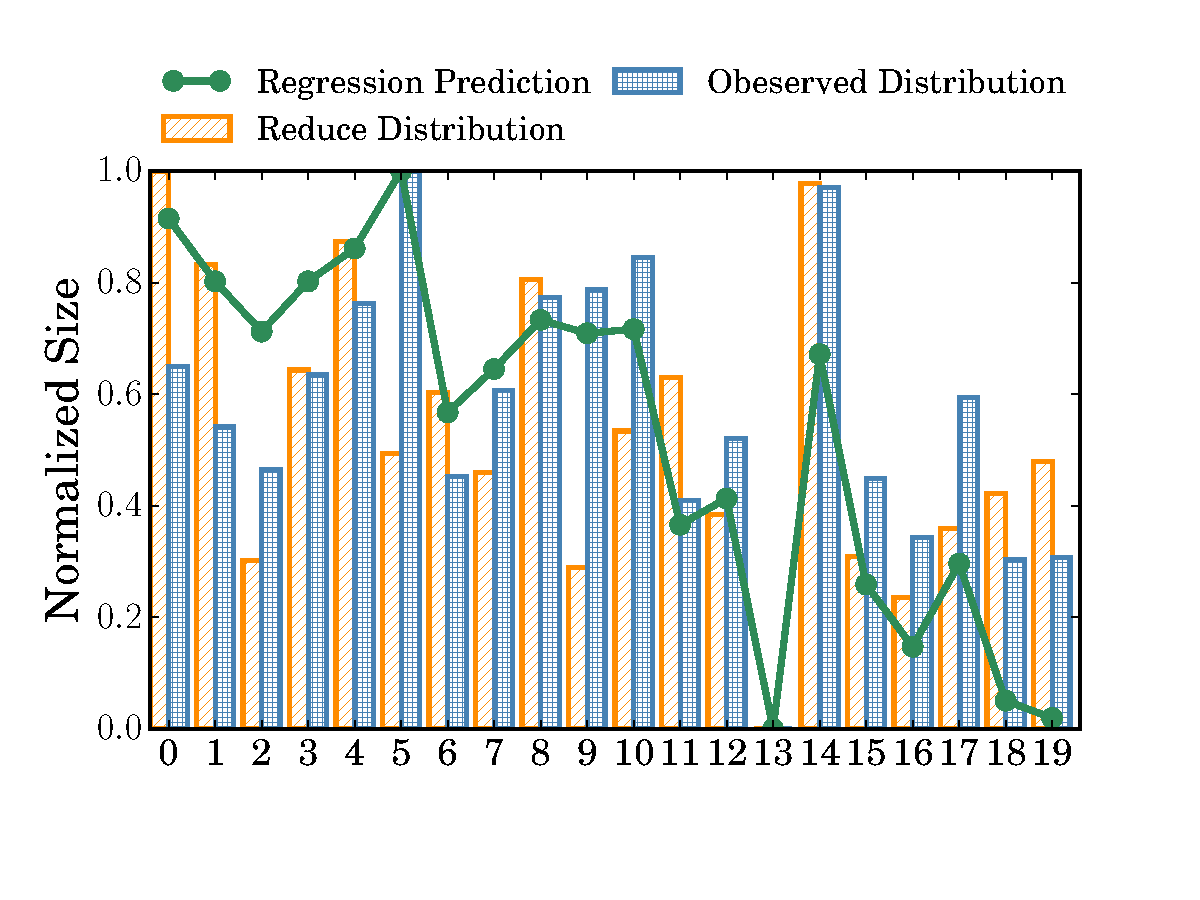
\includegraphics[width=\linewidth]{fig/hash_pre}
		\caption{Linear Regression Prediction of Hash Partitioner}
		\label{fig:hash_pre}
	\end{subfigure}
	\begin{subfigure}[b]{0.32\linewidth}
		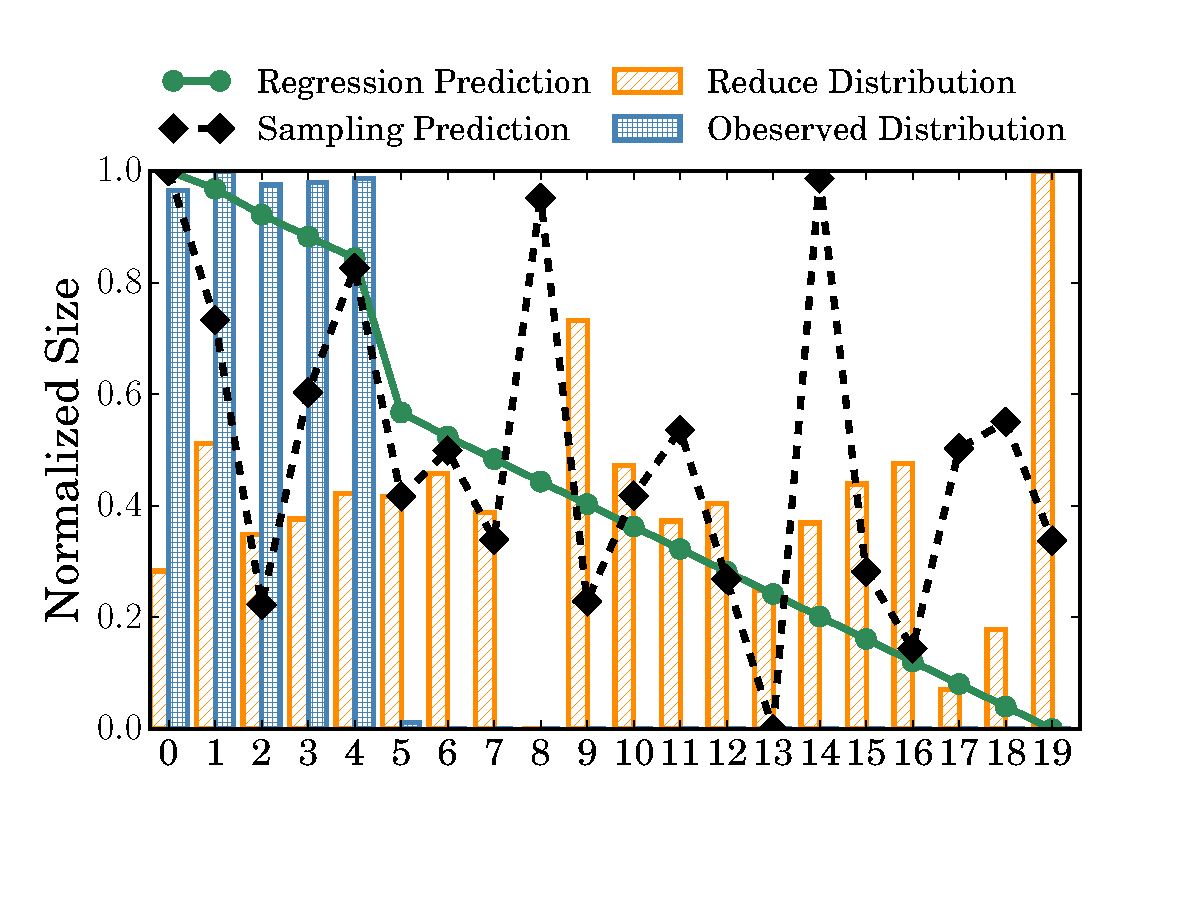
\includegraphics[width=\linewidth]{fig/range_pre_sample}
		\caption{Linear Regression and Sampling Prediction of Range Partitioner}
		\label{fig:range_pre_sample}
	\end{subfigure}
	\begin{subfigure}[b]{0.32\linewidth}
		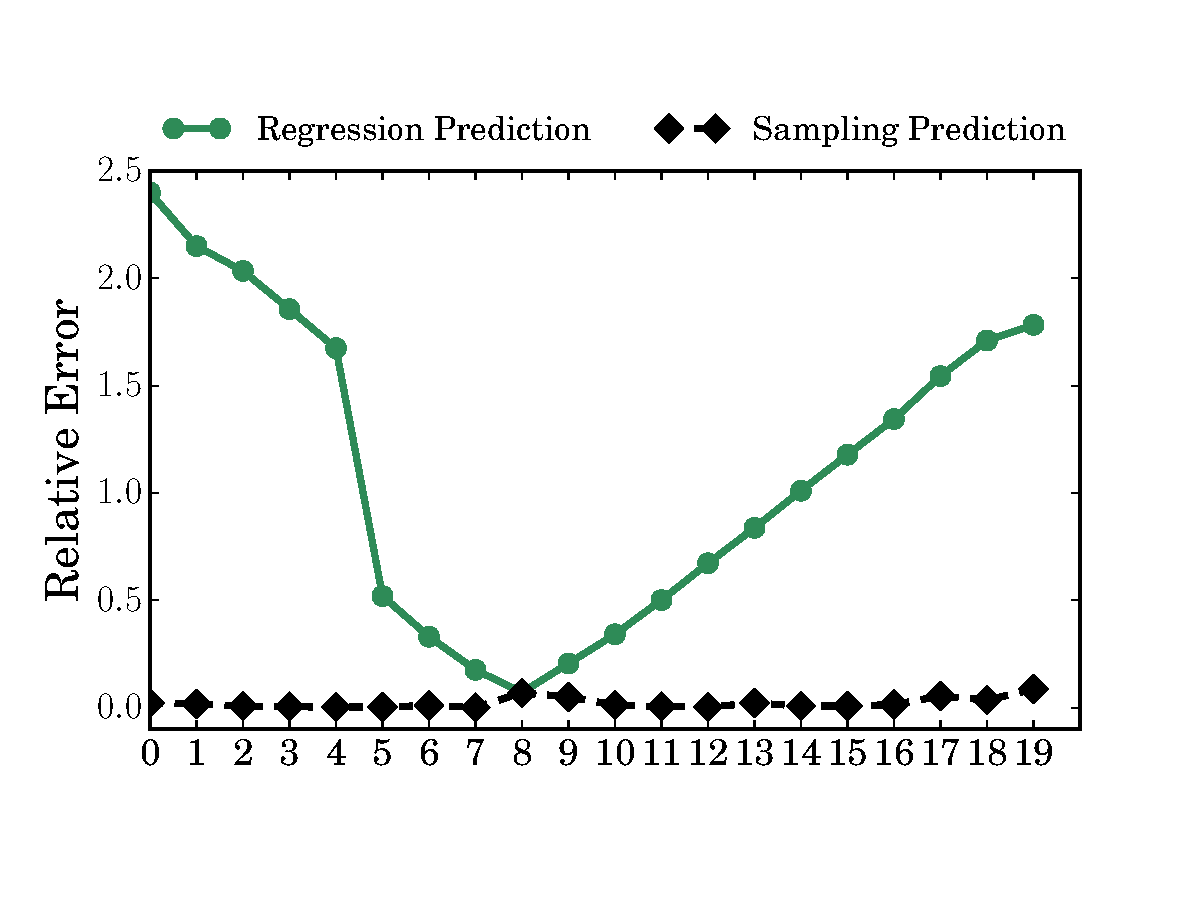
\includegraphics[width=\linewidth]{fig/prediction_relative_error}
		\caption{Prediction Relative Error of Range Partitioner}
		\label{fig:prediction_relative_error}
	\end{subfigure}
	\caption{Reduction Distribution Prediction}
	\label{fig:dis}
\end{figure*}
\subsubsection{Cope with Multiple Shuffles}
Unlike Hadoop MapReduce, multiple shuffles commonly exist in DAG computing. The techniques mentioned in Section \ref{shuffleprediction} can only handle the ongoing shuffle. For those pending shuffle, it's impossible to predict the size. Let all map tasks of shuffle to be scheduled by DAG framework simultaneously can relieve the dilemma. But doing this introduces extreme overhead such as redundant extra task serialization. To avoid violating the optimization from framework, we present Algorithm \ref{mhminheap} to cope with multiple shuffles.

As illustrated in pseudo code \ref{mhminheap}, the size of reduce on each node of previously scheduled $shuffles$ are counted. When a new shuffle starts, the $mSchedule$ is called to schedule the new one with previous $shuffles$. The $size$ of each reduce and its corresponding $porb$ and $host$ are updated by add $p\_reduces$ of new start shuffle. Then the $schedule$ is called to perform the shuffle scheduling. When the new task --- node mapping is available, for each reduce task, if the new scheduled host in $M$ is not equal to the original one, the re-shuffle will be triggered to transfer data to new host for further computing. This re-shuffle is rare since the previously shuffled data in one reduce contributes a huge composition. It means in the schedule phase, the $swap-task$ can help revise the scheduling to match the previous mapping in $shuffles$ as much as possible while maintaining the good load balance.
\begin{minipage}{\columnwidth}
\begin{algorithm}[H]
\caption{Accumulate Scheduling for Multi-Shuffles}
\label{mhminheap}
	\begin{algorithmic}[1]
	\small
	\Procedure{mSchedule}{$m, h, p\_reduces, shuffles$}
		\State
		\Comment $shuffles$ is the previous array of reduce partition ID, host ID and size
		\ForAll{$r\_id$ in $p\_reduces$}
		\State $p\_reduce\left[r\_id\right].size\gets p\_reduce\left[r\_id\right].size + shuffles\left[r\_id\right].size$
		\If{$shuffles\left[r\_id\right].size\geq p\_reduce\left[r\_id\right].size * p\_reduce\left[r\_id\right].prob$}
		\State Update $prob$, set $host$ to $shuffles\left[r\_id\right].host$
		\EndIf
		\EndFor
		\State $M\gets$ schedule$\left(m, h, p\_reduecs\right)$
		\ForAll{$host$ in $M$}
			\ForAll{$r\_id$ in $host$}
				\If{$host\neq shuffles\left[r\_id\right].host$}
				\State Re-shuffle data to $host$
				\State $shuffles\left[r\_id\right].host\gets host$
				\EndIf
			\EndFor
		\EndFor
		\Return $M$
	\EndProcedure
	\end{algorithmic}
\end{algorithm}
\end{minipage} 